\icode{N-EXE-FI-L2-260625-001}
某同学想要了解导线在质量相同时，电阻与截面积的关系，选取了材料相同、质量相等的5卷导线，进行了如下实验：
  
(1)用螺旋测微器测量某一导线的直径如图所示。读得直径\(d =\)\underline{\hbox to 5em{}}\,\qty{}{mm}。

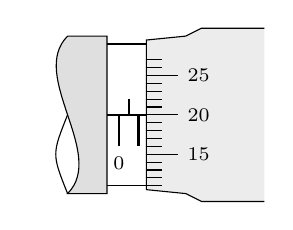
\begin{tikzpicture}[scale=1]
    \filldraw[fill=gray!15] (1.5,-1.1)--(.7,-1.1)--(.5,-1)--(0,-.95)--(0,.95)--(.5,1)--(.7,1.1)--(1.5,1.1);
    \draw (0,.9)--(-.5,.9) (0,-.9)--(-.5,-.9);
    \foreach \y in {-.9,-.8,...,.7}
        \draw[thin] (0,\y)--++(.2,0);
    \draw[thin,font=\scriptsize] (0,0)--(.4,0)node[right]{\(20\)} (0,-.5)--(.4,-.5)node[right]{\(15\)} (0,.5)--(.4,.5)node[right]{\(25\)};
    \draw[thick] (0,0)--(-.5,0) (-.35,0)--(-.35,-.4)node[below,font=\scriptsize]{\(0\)} (-.225,0)--(-.225,.2) (-.1,0)--(-.1,-.4);
    \filldraw[fill=gray!25] (-1,1)--(-.5,1)--(-.5,-1)--(-1,-1)..controls(-.5,-.5)and(-1.5,.5)..(-1,1);
    \draw (-1,0)..controls(-1.2,-.5)..(-1,-1);
\end{tikzpicture}

该同学经实验测量及相关计算得到如下数据：

\begin{table}[ht]
    \centering
    \begin{tblr}{|r|c|c|c|c|c|}
    \hline
    电阻\(R\)/\qty{}{\ohm}&121.0&50.0&23.9&10.0&3.1\\
    \hline
    导线直径\(d\)/\qty{}{mm}&0.801&0.999&1.201&1.494&1.998\\
    \hline
    导线横截面积\(S\)/\qty{}{mm^2}&0.504&0.784&1.133&1.753&3.135\\
    \hline
    \end{tblr}
\end{table}

(2)请你根据以上数据判断，该种导线的电阻\(R\)与截面积\(S\)是否满足反比关系?若满足反比关系，请说明理由;若不满足，请写出\(R\)与\(S\)应满足的关系。

(3)若导线的电阻率\(\rho =\) \,\qty{5.1e-7}{\ohm\cdot m}则表中阻值为\,\qty{3.1}{\ohm}的导线长度\(l =\) \underline{\hbox to 5em{}}(结果保留两位有效数字)。